\section{Paralelización de un algoritmo de procesamiento digital de imágenes.}

Se nos pide paralelizar un algoritmo de procesamiento de imágenes que aplica una misma
matriz de convolución de dimensión 3x3 a todos los píxeles de una imagen, a excepción de los bordes. La
gestión de los bordes depende de la política que queramos aplicar por lo que escapa de
los intereses del ejercicio.
\subsection{Solución propuesta.}

Al tener como restricción el que la paralelización del algoritmo
se realiza a nivel de proceso decidimos realizar un particionamiento de carga en base
a datos. Concretamente dividimos las filas de la imagen entre el número de procesos, de forma
que las filas correspondientes a cada proceso son contiguas y de forma que las filas
sobrantes de la partición y las no paralelizables las trata el proceso principal.

El algoritmo requiere tanto de una matriz de convolución como de un conjunto de pixeles de entrada
(a procesar) y otro de salida. Para comunicar la matriz de convolución a los distintos procesos
utilizamos \texttt{MPI\_Broadcast}.
Para transmitir y recibir los conjuntos de píxeles (filas) hacemos uso de la funcion \texttt{MPI\_Scatter}, la cual a partir
de un segmento contiguo de memoria realiza una partición de la longitud que se le indique enviando cada
parte a cada proceso del grupo de comunicación que se le indique, y su complementaria \texttt{MPI\_Gather}.

Elegimos esta solución por diversas razones:

\begin{enumerate}
    \item Estas funciones están preparadas para escalar según el número de procesos \cite{MPIBroadcast}.
    \item Aunque \texttt{MPI\_Scatter} requiere que la memoria no se solape, haciendo que por cada par de
    procesos haya una linea que tiene que tratar el proceso cero, preferimos esto a complicar el código.
    \item Desconocemos dónde residen los cuellos de botella y no consideramos adaptar la solución
    a la naturaleza del hardware subyacente.
\end{enumerate}

Podemos obtener los detalles de la implementación en el fichero adjunto \texttt{ejercicio\_2.c}, donde en
la función \texttt{convolucion\_paralelizada} relatamos los pasos que seguimos.

Para comprobar que el algoritmo da resultados correctos realizamos una prueba que consiste en procesar una imagen una vez con el algoritmo
que se nos proporciona y otra con nuestro algoritmo paralelizado, comprobando que ambas coincidan. Podemos ejecutar estas pruebas con \texttt{make test}.

\subsection{Evaluación del algoritmo paralelizado.}

Una vez que comprobamos que el algoritmo es correcto ejecutamos el script \texttt{benchmark.sh} que nos proporciona
información acerca de los tiempos de ejecución y del tiempo de CPU consumido. Podemos ver esta información representada
en las siguientes figuras.

\begin{table}[!ht]
    \centering
    \begin{tabular}{|l|l|l|}
    \hline
        \textbf{nprocs} & \textbf{wall\_time} & \textbf{cpu\_time} \\ \hline
        1 & 1,262646 & 1,259698 \\ \hline
        2 & 0,659454 & 2,627602 \\ \hline
        3 & 0,460211 & 4,073324 \\ \hline
        4 & 0,367742 & 5,507351 \\ \hline
        5 & 0,319758 & 7,114452 \\ \hline
        6 & 0,296706 & 9,049741 \\ \hline
    \end{tabular}
    \caption{Tabla con los tiempos de ejecución obtenidos para el \textit{benchmark} \texttt{nitori\_get\_down.pgm} en un \texttt{Macbook Pro}
    con un procesador Intel \texttt{i7-9750H}. A simple vista podemos observar cómo, aproximadamente, el tiempo
    transcurrido se va dividiendo por el número de procesos, mientras que el tiempo empleado por la CPU se va
    multiplicando por el número de procesos más un tiempo que aumenta progresivamente.}
\end{table}


\begin{figure}[H]
    \centering
    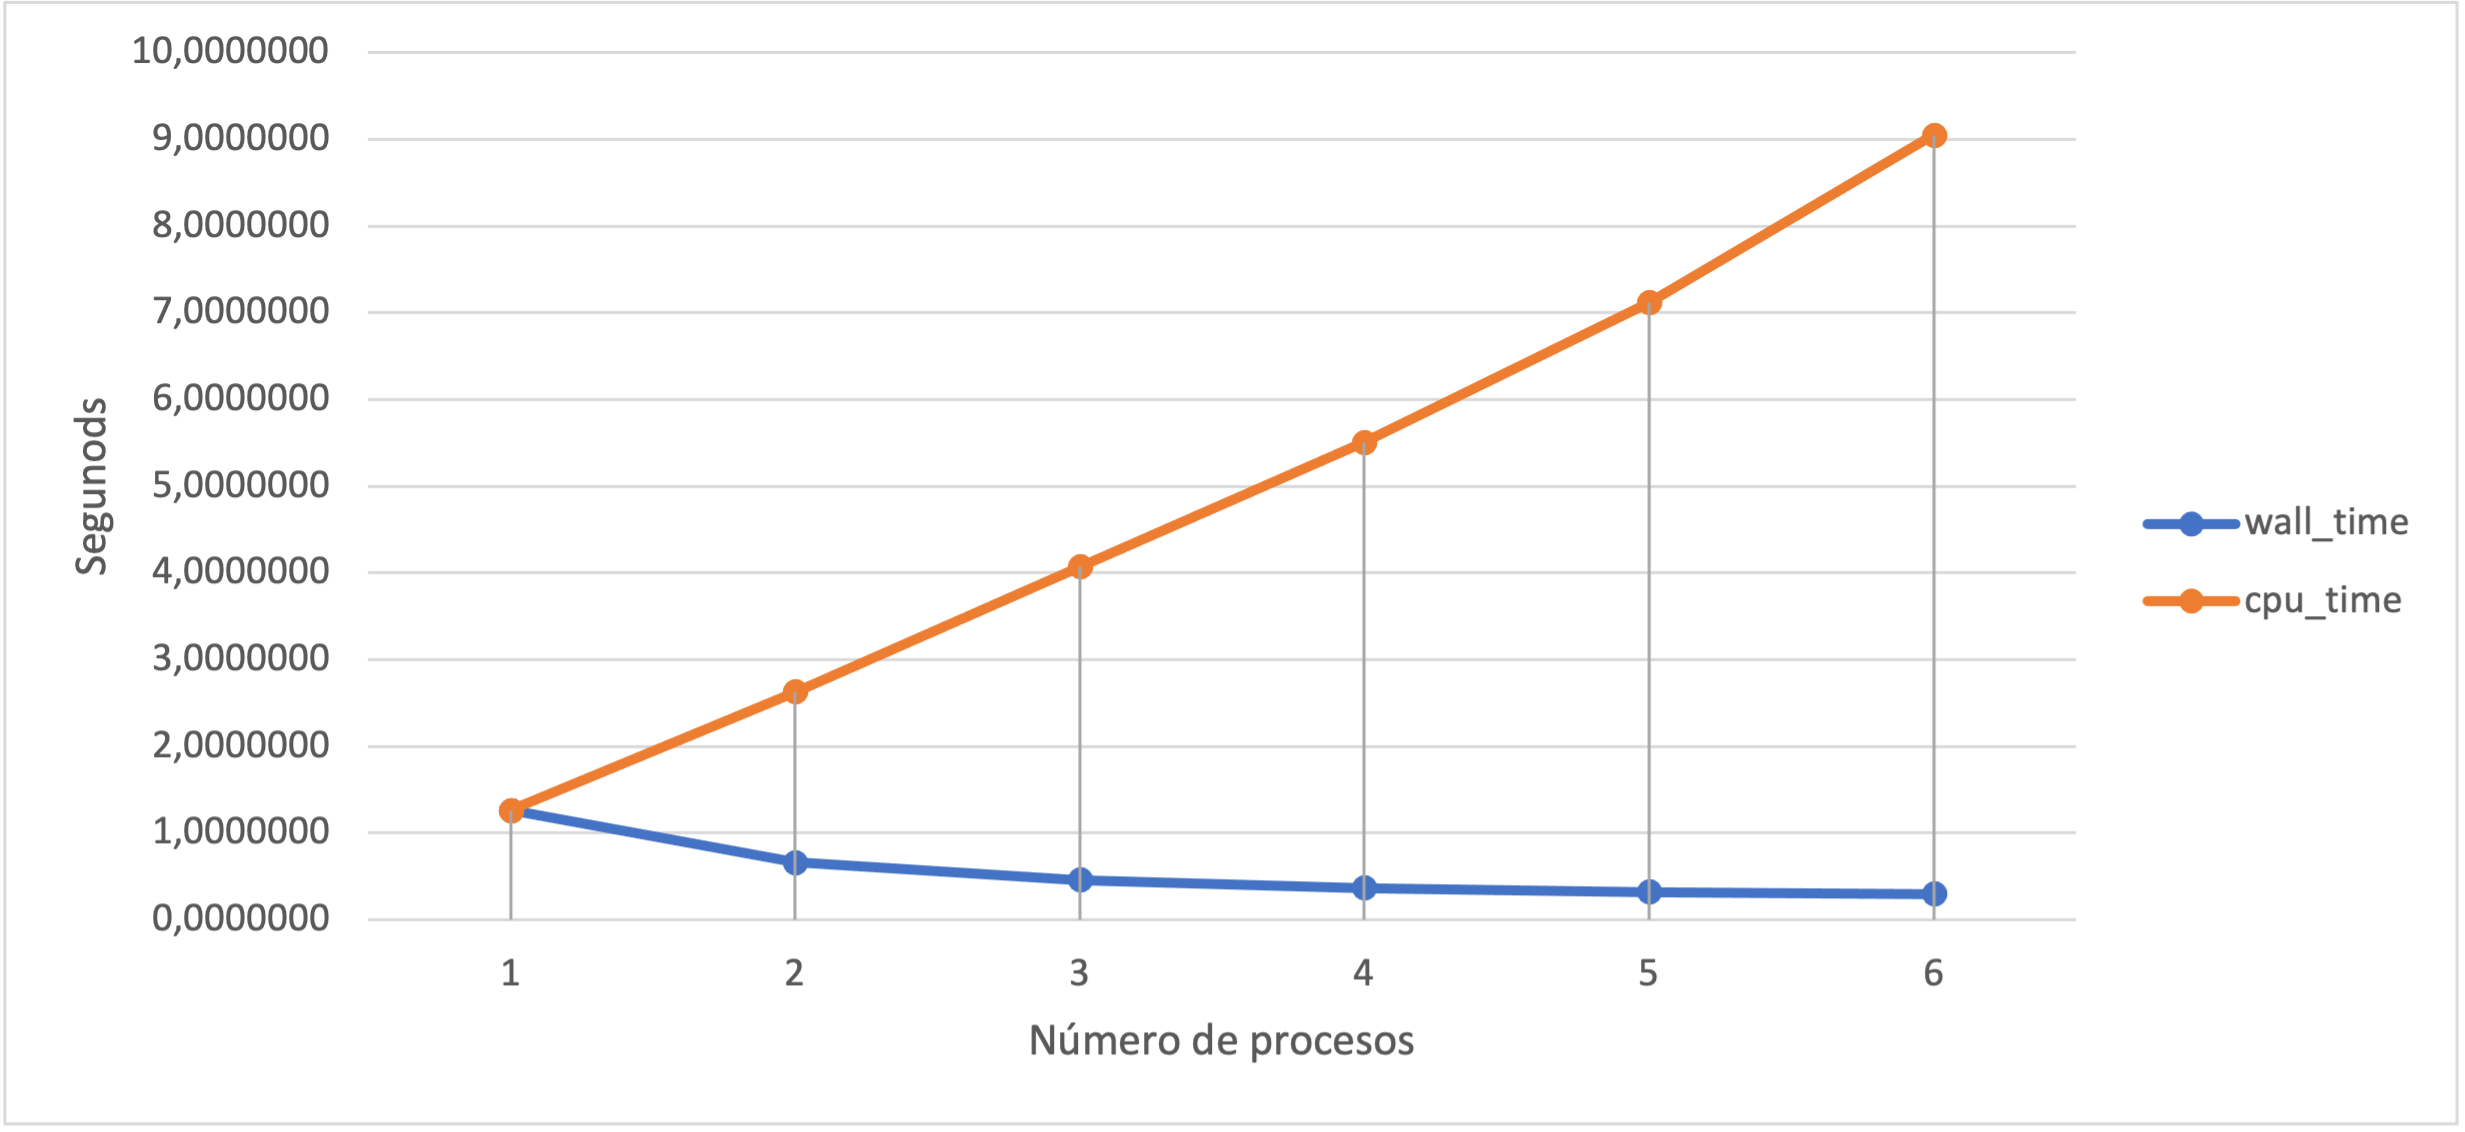
\includegraphics[width=\textwidth]{nitori_segundos_nprocs.png}
    \caption{Relación Segundos/Número de procesos para los resultados obtenidos en el \textit{benchmark} \texttt{nitori\_get\_down.pgm}.
    Vemos la relación entre los recursos utilizados con respecto a la mejora de ejecución en tiempo transcurrido.}
\end{figure}

\begin{figure}[H]
    \centering
    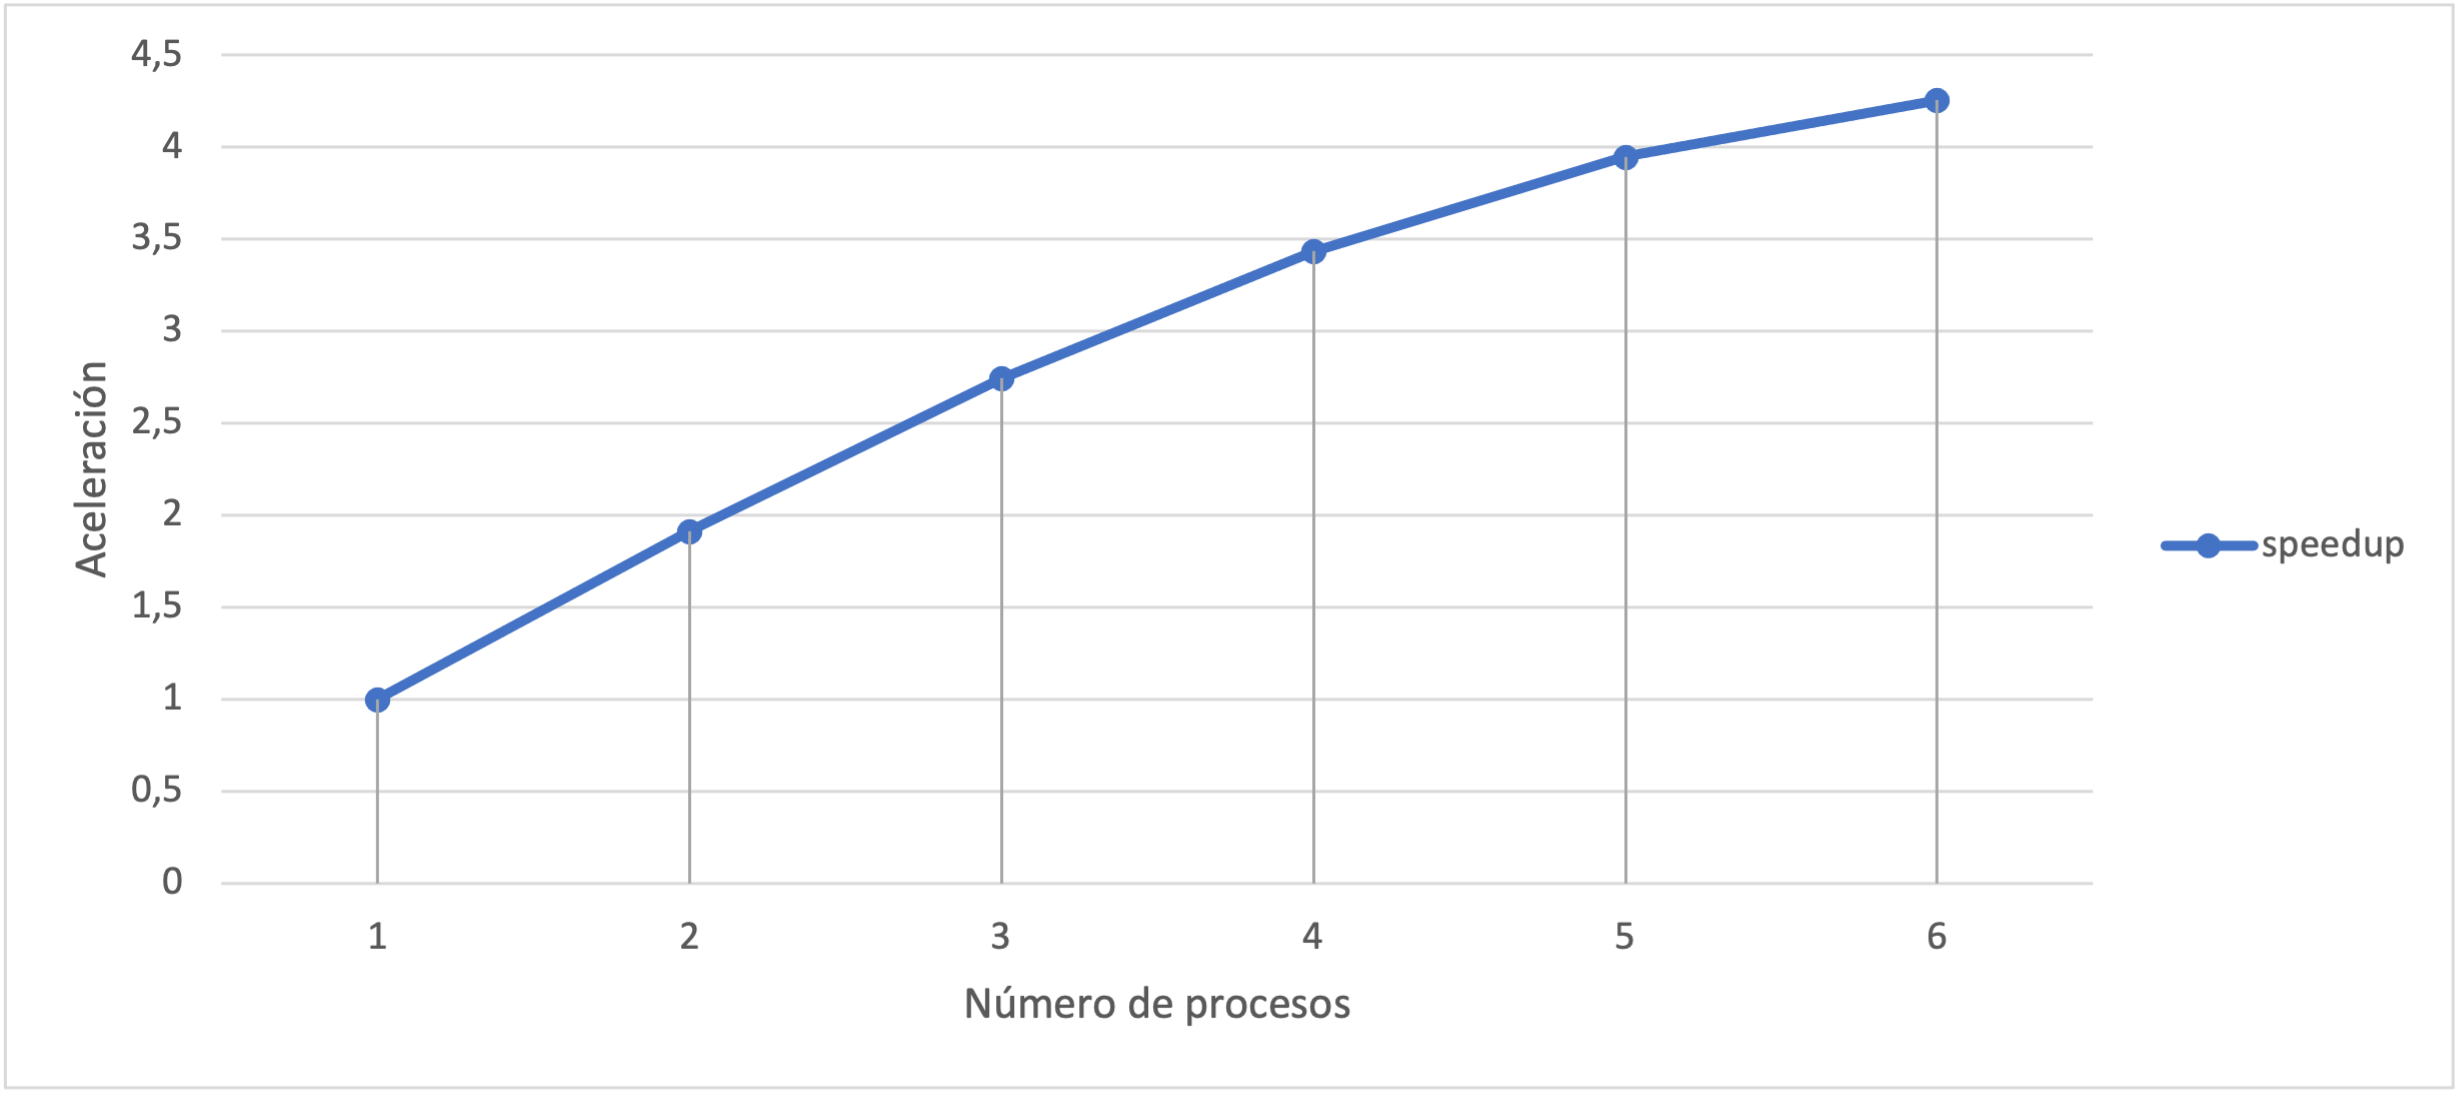
\includegraphics[width=\textwidth]{nitori_speedup_nprocs.png}
    \caption{Relación factor de Aceleración/Número de procesos para los resultados obtenidos en el \textit{benchmark} \texttt{nitori\_get\_down.pgm}.
    Podemos observar cómo este crecimiento no es lineal según aumenta el número de procesos, sino que sigue una curva determinada tanto por el \textit{overhead}
    resultante de paralelizar el algoritmo como por las partes no paralelizadas en el algoritmo.}
\end{figure}

\subsection{Trabajo futuro.}

Si necesitásemos optimizar más el algoritmo el primer paso sería identificar el problema a resolver. Para ello nos
podríamos servir de herramientas de \textit{profiling}, investigando datos relevantes como ciclos de reloj ociosos,
número de fallos de caché, funciones con mayor carga de trabajo, etc. Una vez identificados los puntos a optimizar
se podría mejorar la solución propuesta o proponer otra.
